\section{A place for everything ...} \label{sec:Variables}

Programming is, at it's heart, about manipulating data. That data needs to be stored in the computer in such a way that we know what it is. Consider the following block of text.

\begin{quote}
    \textbf{Colin} is a \textbf{Lecturer} in the department of \textbf{Computer Science}. They have a class of \textbf{2} students studying \textbf{Python}. The course starts on the \textbf{19th of September} and runs for \textbf{3} days. The names of the students are \textbf{Alex Smith and Charlie Jones}.
\end{quote}

The structure of the block tells us something about how the values in bold interact. We can consider each item in bold as a placeholder for a value that could be changd without changing the intention of the text with is to inform you about someone's role and teaching responsibilities. So if we change only the values we might get something like this.

\begin{quote}
    \textbf{Tracy} is a \textbf{Senior Lecturer} in the department of \textbf{Philosophy}. They have a class of \textbf{3} students studying \textbf{Ethics}. The course starts on the \textbf{24th of October} and runs for \textbf{2} days. The names of the students are \textbf{Bob, Carlos and Aled}.
\end{quote}

You might think of the structure of the text block as a program.


Fire up the python interpreter in a command (or terminal)  window and type in the following commands. The print command is one we will use quite a bit in this course, simply type print then put what you want to output in the brackets.

\begin{python}[]
>>> print("Colin")
>>> print(4)
>>> print(3.5)  
>>> print("Colin is a Lecturer in the department of Computer Science")
\end{python}

Notice that event though you have put quotation marks around some of the values the quotes don't show in the output. That's because we are using the quotes to tell Python than the thing we are dealing with is a string of text character. 

Indeed we can ask Python about what type of thing we are dealing with using the type function\footnote{We are using functions here, don't worry too much about that for now as we will get to them in a later chapter. For now simply type what is written and check that you match the brackets.}. So try typing each of the following in turn:

\begin{python}[]
>>> type("Colin")
>>> type(4)
>>> type(3.5)
>>> type("3.5")
\end{python}


So we are being told that ``Colin" is a string (<class 'str'>), 4 is an integer (<class 'int'>), 3.5 is a floating point number (<class 'float'>), and ``3.5" is a string (<class 'str'>). Just think about that last one for a moment. Putting quotes round a number turns it into a string. Why does that matter? Well let's take a look at what happens if we try and use this value in a mathematical equation. Type the following and try to explain what the program is doing\footnote{Note that you are only typing the bits preceded by >>>, the text on the other lines is the response from the Python interpreter.}.

\begin{python}
>>> print(3+4)
7
>>> print(3*4)
12
>>> print("3"+"4")
34
>>> print(3*"4")
444
>>> print("3"*"4")
Traceback (most recent call last):
  File "<stdin>", line 1, in <module>
TypeError: can't multiply sequence by non-int of type 'str'
\end{python}

The first two lines are simple arithmetic and we get returned the answers 7 and 12 for addition and multiplication respectively. The third line is interesting as Python is trying to be helpful. We can't "add" two strings together but it is quite common for people to want to concatenate strings so the people who developed Python decided the "+" symbol could be a nice shorthand way of doing this so ``3"+``4" = ``34". Similarly on the 4th line Python reads this as meaning you want to duplicate the string 3 times so 3*``4" = ``444". Finally on the last line we are asking Python to multiply two string, unfortunately even Python doesn't know what you are asking for here and simply returns an error giving you a possible suggestion of how you went wrong.

\subsection{Variables}

Having looked at how Python works with values let's  consider a closely related idea, that of variables. Consider once again our text in the previous section and think about writing the block in a form where name of the lecturer might change. Here we would want to put a placeholder in for the name that we can set to be anything when the program is run. This placeholder is called a variable.

Look at the following code and see if you can work out what it will do before you run it.

\begin{python}
>>> name = "Colin"
>>> print("The lecturer is called ", name)
>>> print(name," works in the Department of Computer Science")
\end{python}

What we have done is created a variable called \emph{name} and stored a string in it that we will use later. In fact having started the value in a variable we can use it many times in lots of different places.

In fact you can ask the user to give you a value to use in your code. This makes use of the input command which is a little bit like the print command. Try the following.

\begin{python}
>>> name = input("What is your name? ")
>>> print("Hello ", name, " nice to meet you".)
>>> answer = input(name," what is your favourite colour?")
>>> print("Nice!, ",name,". ",answer," is my favourite colour too")
\end{python}

Question : What is the variable type for answer?

If you said string, then well done, but what happens if we don't want a string? What happens when we want a number. Well luckily Python gives us functions that allow us to change the type of a variable. Try the following.

\begin{python}
>>> int("3")
>>> float("3.5")
>>> int("3.5")
>>> str(3.5)
>>> int("Fred")
\end{python}

Notice that we can turn any number into a string, but we can't turn any string into a number. You should also be aware that making a number an integer will throw away the decimal part.

\subsection{Writing larger programmes}

So far we have largely been looking at simple Python commands in isolation but the real power in programming comes when we link commands together to under achieve more complex tasks.

Let's consider a simple mathematical problem. Calculating the length of a side for a triangle when we are given 2 sides and the angle between them. we know that this problem can be solved using the cosine rule as shown below. 



    \begin{center}
        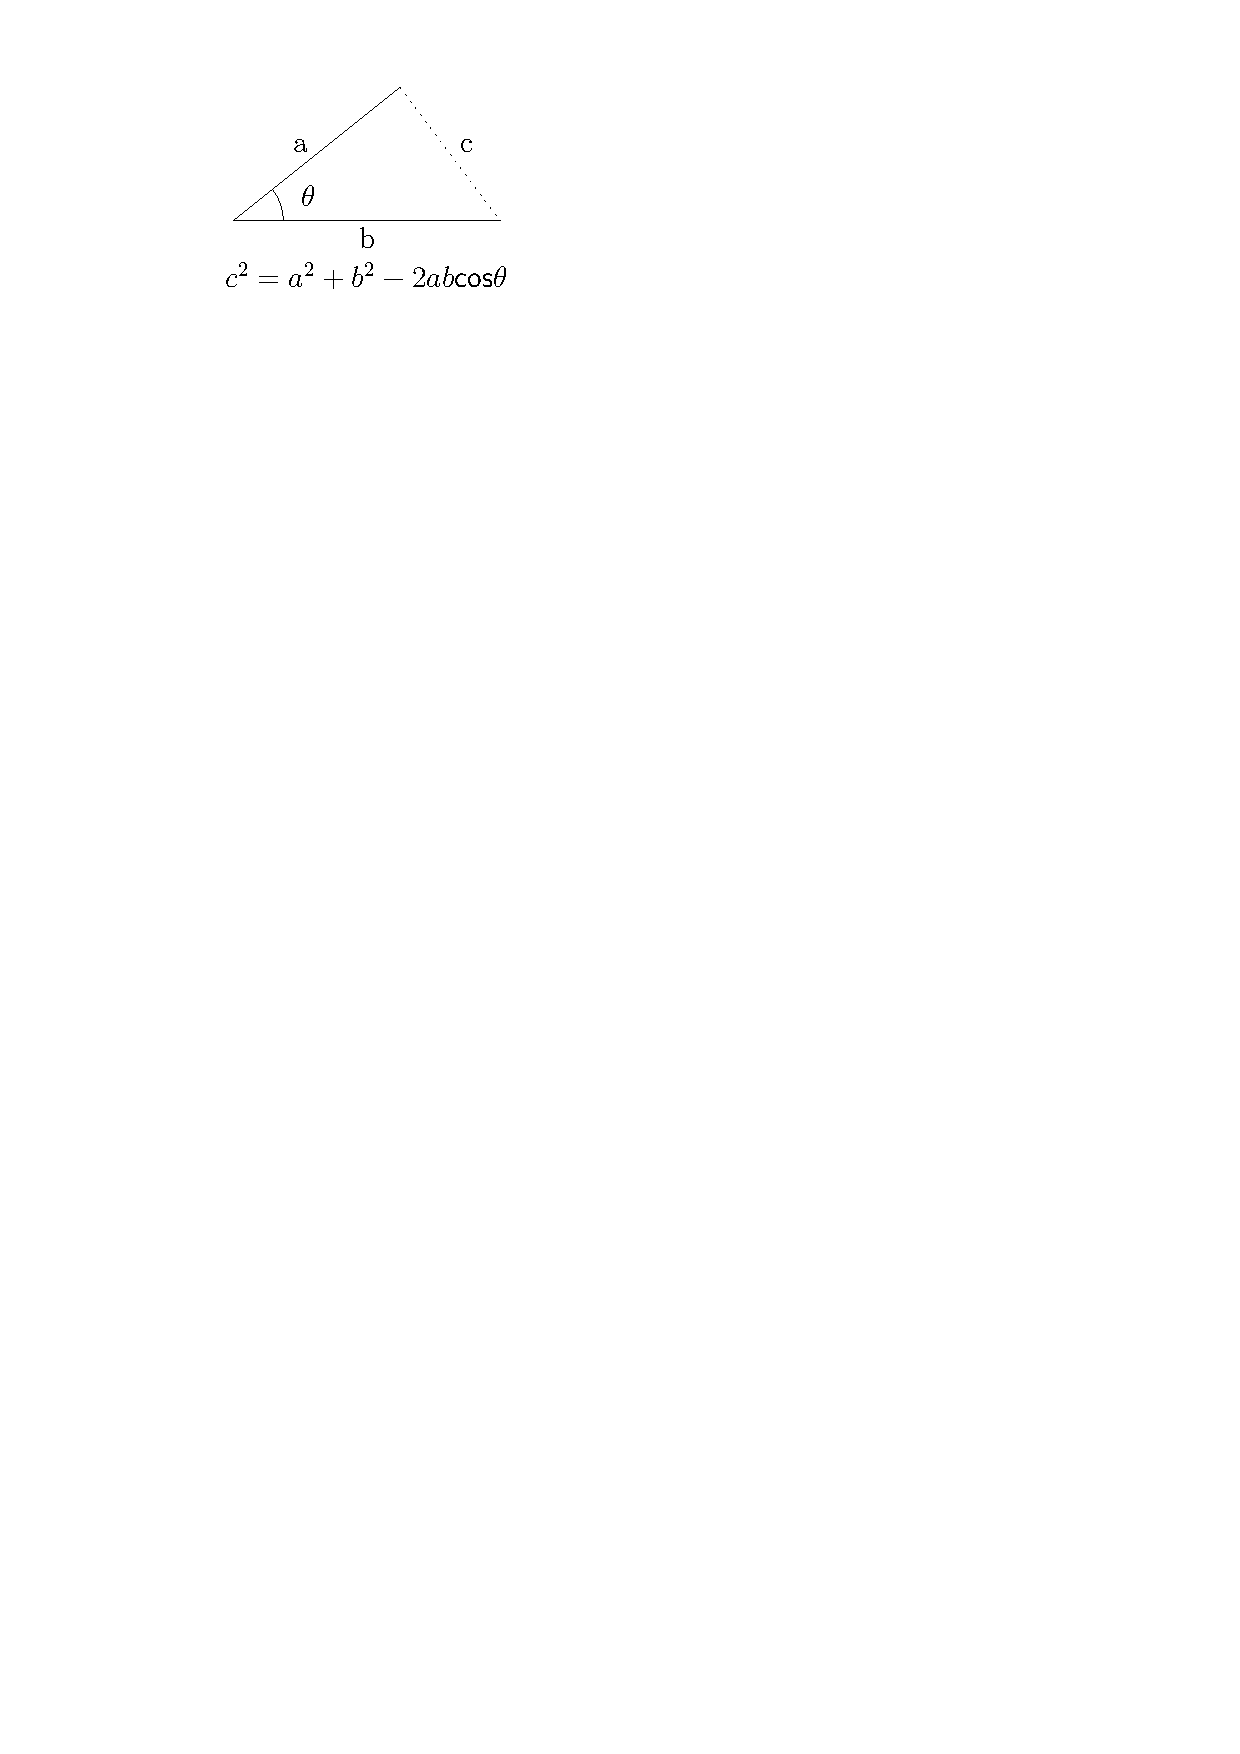
\includegraphics[width=0.3\linewidth]{images/cosineRule.pdf}
    \end{center}

Before we start to write our program let's think about the steps we will need to under take to solve this problem:
\begin{enumerate}
\item Get the length of the sides and the angle from the user
\item Because these will be strings we will need to convert them to numbers so we can do the maths.
\item We will get the angle in degrees but the cos function expect radians so we will need to convert it.
\item Apply the cosine rule
\item Display the length of the side.
\end{enumerate}

This process of breaking a problem down before you start writing is crucial to writing computer programs and it's something I often do with pen and paper before even opening the editor. So having written down the steps we need to take, now open up VSCode and create a program called ``Traingles.py". Once open type in the following program, note that I have included line numbers to help me explain the program, you do not need to type them.

\begin{minipage}{\textwidth}
\lstinputlisting[language=Python,
    basicstyle=\sffamily\footnotesize,
    keywordstyle=\textbf, 
    commentstyle=\color{blue},
    showstringspaces=false,
    frame=tb, 
    numbers=left,  
    label={lst:PythonCode}]{Python/Triangles.py}
\end{minipage}

\textbf{Comments:} are used to explain what it going on in the code and is particularly important if you are sharing your code with others or if you might return to the code later, wen you will have forgotten your design decisions. In the program shown comments are added in two ways. In Lines 1 -- 5 a multi-line comment is started, and finished, with three quotation marks. This type of comment is common at the beginning of blocks of code to explain the rationale for the next section. Lines 7,8,11 etc. use a hash mark (\#) and are used for short, single line, comments.

\textbf{Libraries:} Line 9 shows an example of including a library. Libraries are key to the power of Python and we will learn more about them as we progress through the book, but for now just understand that including a library gives us access to functionality that is not in the core language. In this case we are saying we are going to use mathematical functions (like cosine). Having imported the library can then use the ``math" to access values and functions defined in the library, e.g. ``math.pi" and ``math.cos(...)".

\textbf{Formatted Printing:} I've also taken this program as an opportunity to introduce to you formatted printing. We have already come across the print function, but here it's slightly different. Inside the brackets I have used the letter ``f" directly before the string to say this is a formatted string. This means that wherever there are curly brackets in the string it means I want you to replace this with the value stored in a variable. e.g. ``print(f``{name}")" means print out the value stored in the ``name" variable.

\textbf{Readability:} You might be tempted to combine lines to shorten the program. This is of course possible, but be warned, simple is good when it comes to maintaining code. Trying to fix a complicated programme might take more time than writing it did in the first place.

Consider the following program which does the same as Triangles.py. I hope you can see that whilst the functionality is exactly the same the choices we made in layng out the code impact our ability to digest what is doing wrong.

\begin{minipage}{\textwidth}
\lstinputlisting[language=Python,
    basicstyle=\sffamily\footnotesize,
    keywordstyle=\textbf, 
    commentstyle=\color{blue},
    showstringspaces=false,
    frame=tb, 
    numbers=left,  
    label={lst:PythonCode}]{Python/Triangles2.py}
\end{minipage}

\subsection{Collections}

So far we have only considered 3 simple data types i.e. integers, floating point numbers and strings. In this next section we will look at variables that can hold a number of objects in a collection.

\textbf{Lists:} We will start our exploration of collections by looking at lists. A list can hold a number of things in order and each thing need not be of the same type. 

Open your python interpreter (in a terminal or command window) and type the following:

\begin{python}
>>> students = ["Alex", "Charlie", "Sam"]
>>> marks = [67, 58, 84]
>>> mixed_list = [1, "first", "primary", 1.0]
\end{python}

In each case we have created a single value that has multiple values. To use a value stored in the variable we need to tell python which element of the list we are interested in. We do this using the square brackets and an integer index, starting at 0. Try the following:

\begin{python}
>>> students[0]
'Alex'
>>> marks[2]
58
>>> mixed_list
[1, 'first', 'primary', 1.0]
\end{python}

Notice that if we don't specify an index then we get the entire list returned.

Now let's try changing the values in a list:
\begin{python}
>>> students[0] = "Jackie"
>>> mixed_last[3] = "one"
>>> marks[3] = 67
\end{python}

The first two lines changed the value in the list, even though in the second case we were inputting something of a different type. In the final line however we get an error. The problem is that once we have defined a list the size of it is fixed. We will need some clever code (or a new library) to have lists that can change their size once the program is running.

Here's a challenging little question, ``What do you think the following snippet of python will do?" 

\begin{python}
>>> name = "Alex"
>>> my_list = [1, name]
>>> name = "Sam"
>>> print(my_list[1])
\end{python}

Once you have decided type it into the interpreter and see if you were right.


\textbf{Tuples:}

\textbf{Dictionaries:}



\subsection{Some useful bits and pieces}

Boolen Values 

Mult-line strings

Non decimal numbers
